\documentclass{article}
\usepackage[utf8]{inputenc}
\usepackage{natbib}
\usepackage{graphicx}
\usepackage{gensymb}
\usepackage{xspace}
\usepackage{amsmath}
\newcommand{\minus}{\scalebox{0.75}[1.0]{$-$}}
\graphicspath{ {./images/} }

\newcommand{\gera}{\"{a}}
\newcommand{\gero}{\"{o}}
\newcommand{\geru}{\"{u}}
% \newcommand{\gers}{}
\renewcommand{\contentsname}{Inhaltsverzeichnis}
\begin{document}
\begin{titlepage}
    \begin{center}
        \vspace*{4cm}
 
        \Huge
        \textbf{Systemtheorie 2}
 
        \vspace{0.5cm}
        {\huge Inverses Pendel}
       
        \vspace{1.5cm}
 
        \LARGE{Panwei Hu, Hannes Joisten, Tim Rehbronn}
 
        \vfill
 
        \Large
        E.ON Energy Research Center \\
        RWTH Aachen University\\
        Januar 2020
 
    \end{center}
\end{titlepage}
\newpage
\tableofcontents
\newpage

\section{Rotation des Pendels}
\subsection{Aufbau des Modells}
\vspace{5mm}

\begin{figure}[h]
  \centering
  \begin{minipage}[b]{1\textwidth}
    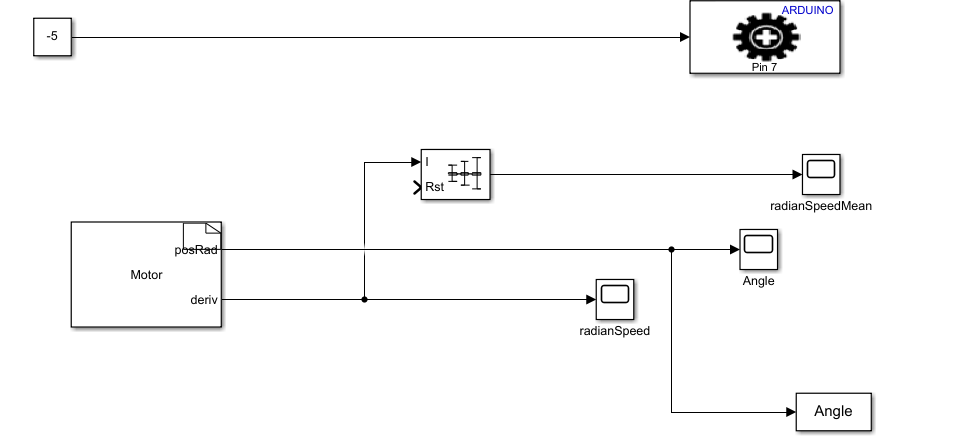
\includegraphics[width=\textwidth]{model.png}
    \caption{Modell Simulink, Stand Aufgabe 1}
  \end{minipage}
\end{figure}
\vspace{5mm}

Das Modell wurde wie oben in Figure 1 zu sehen in Simulink implementiert.
Die Eingabe in das 'Continous Servo Write'-Modul erfolgt mittels eines 'const'-Moduls, wobei 90 die maximale Ansteurungsgröße darstellt.
Weiterhin stellt der bereits vorgegebene Block 'Motor' sowohl die Position des Motors in Radiant als auch die aktuelle Winkelgeschwindigkeit in Radiant/Sekunde.
Ausgelesen wurde diese Geschwindigkeit über Bildung des arithmetischen Mittlewertes.
Die Display Blöcke dienten zur Anzeige und Überwachung der Größen.\\
\\In der oberen Lage hat der Motor eine gemessene Position von $\pm180\degree$. 
\\Das Vorzeichen der Steuergröße gibt die Richtung des Drehmoments und damit der Rotation des Motors vor.
Das Positionssignal des Motors schwingt je nach Auslenkung zwischen 0 und $2\pi$.\\
\newpage

\subsection{Motoranalyse - Brownout}
\vspace{5mm}

\begin{figure}[h]
  \centering
  \begin{minipage}[b]{0.4\textwidth}
    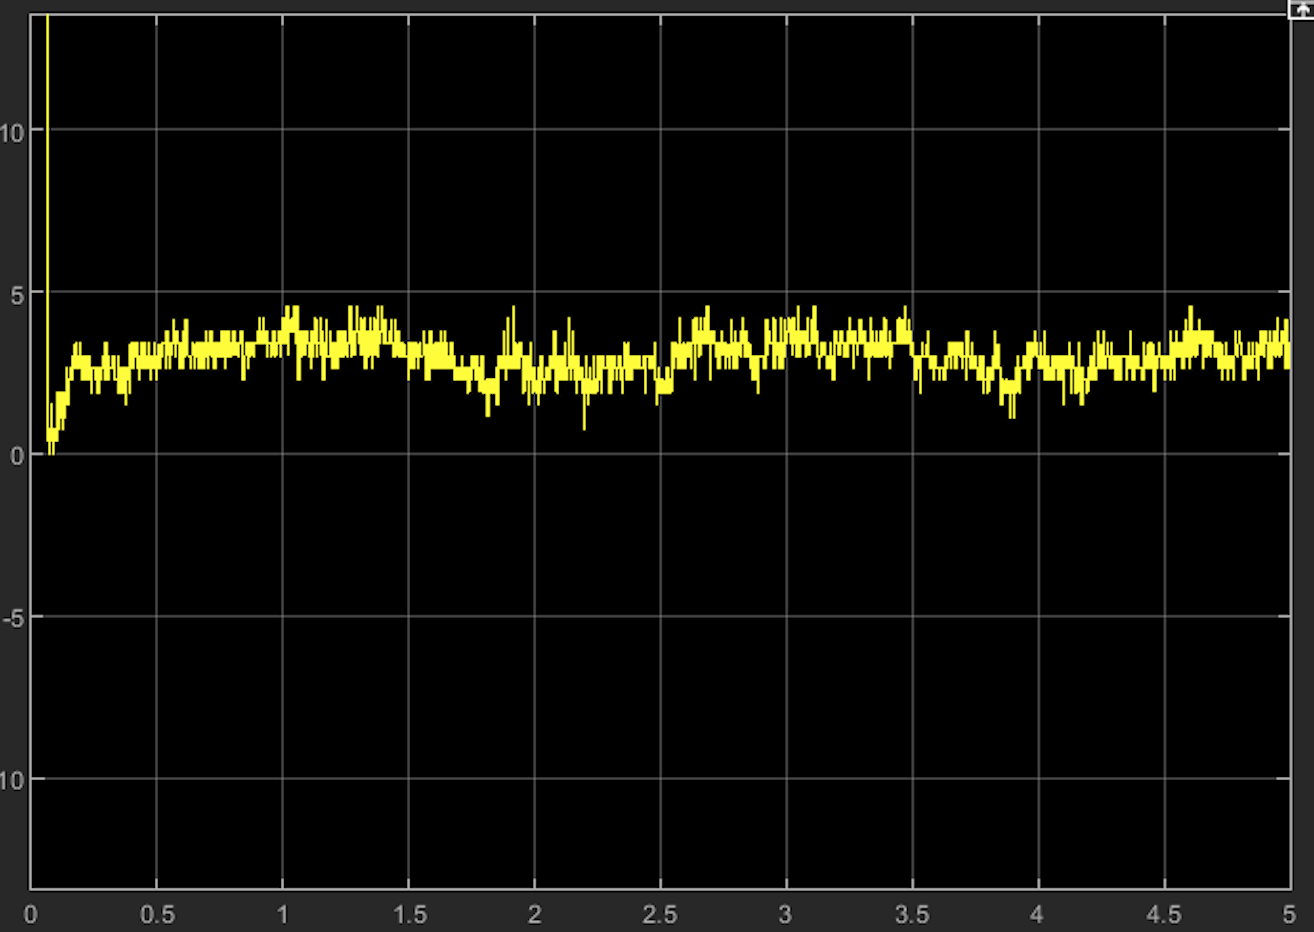
\includegraphics[width=\textwidth]{-5.png}
    \caption{Motorinput = -5}
  \end{minipage}
  \hfill
  \begin{minipage}[b]{0.4\textwidth}
    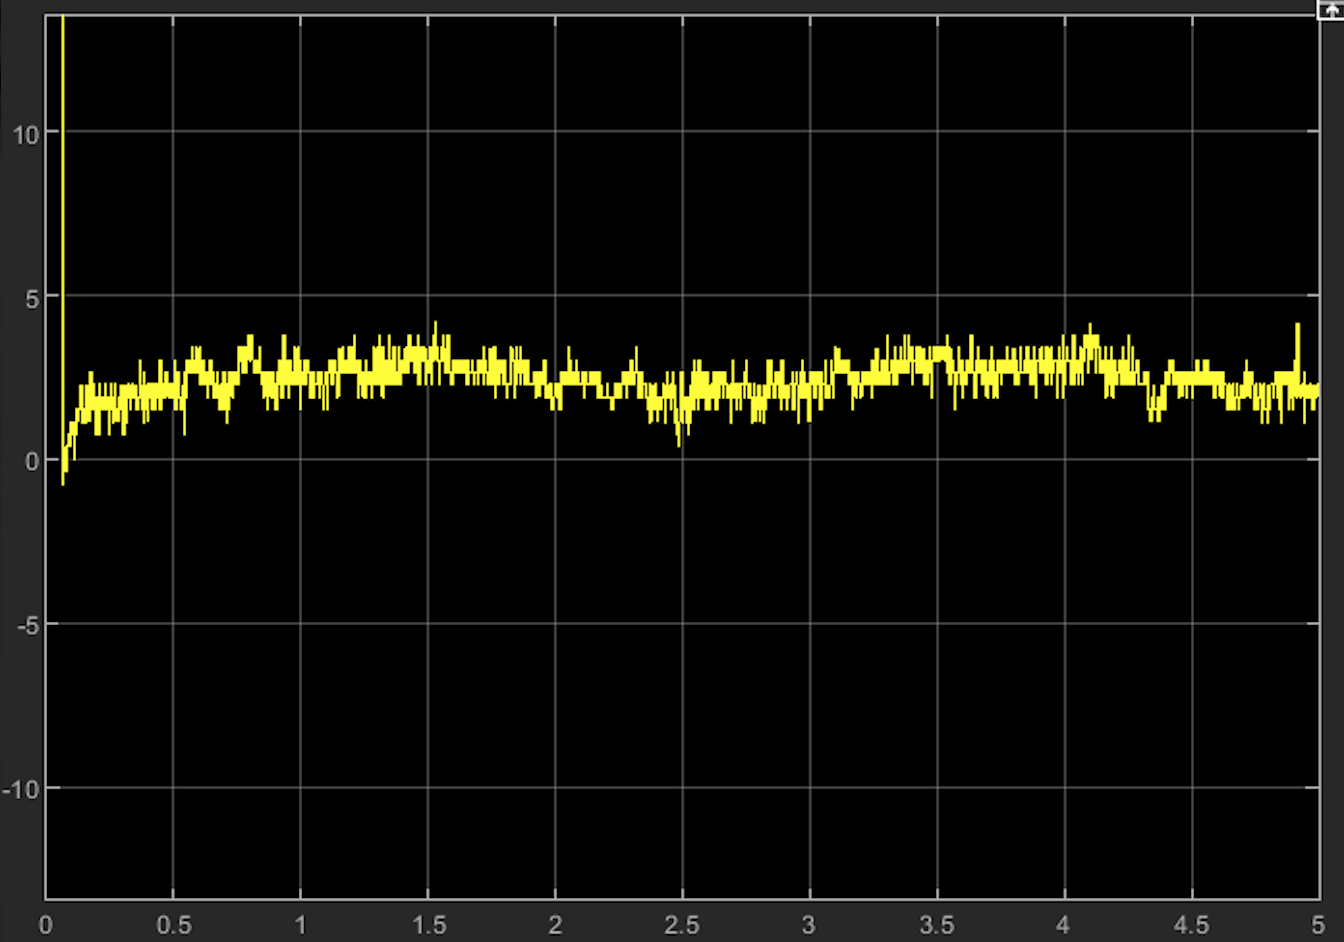
\includegraphics[width=\textwidth]{-4.png}
    \caption{Motorinput = -4}
  \end{minipage}
\end{figure}


\vspace{5mm}

Weiterhin musste der Motor analyisiert werden, um die möglichen Betriebsbereiche zu ermitteln.
Durch eine Intervallsuche fanden wir den positiv gültigen Bereich, also den Bereich, in dem kein Brownout auftritt bei:
\\$10\,< \, \text{Steuergröße} \,< \, 30$\\Der negative gültige gemessene Bereich:\\ $\minus 18\,< \, \text{Steuergröße} \,< \, \minus4$.\\
Hierbei sieht man anhand von Figure 2 und Figure 3, dass zwischen den Motoreingaben keine Veränderung in der Geschwindigkeit der Rotation feststellbar ist - es scheint als eine Grenze gefunden.
Analog beobachteten wir ähnliches für die betragsmäßig maximale unterer Grenze der negativen Eingabe und für den positiven Bereich der Eingabegröße.
Betragsmäßig gibt es also je nach Richtung der Drehung unterschiedlich gültige Bereiche für die Steuergröße. 
Dies liegt an dem Aufabu von Gleichsstrommotoren, was zu Asymmetrischem Verhalten im Aussteuern führt.
\newpage

\subsection{Analyse Winkelpostionssignal}
\vspace{5mm}

\begin{figure}[h]
  \centering
  \begin{minipage}[b]{1\textwidth}
    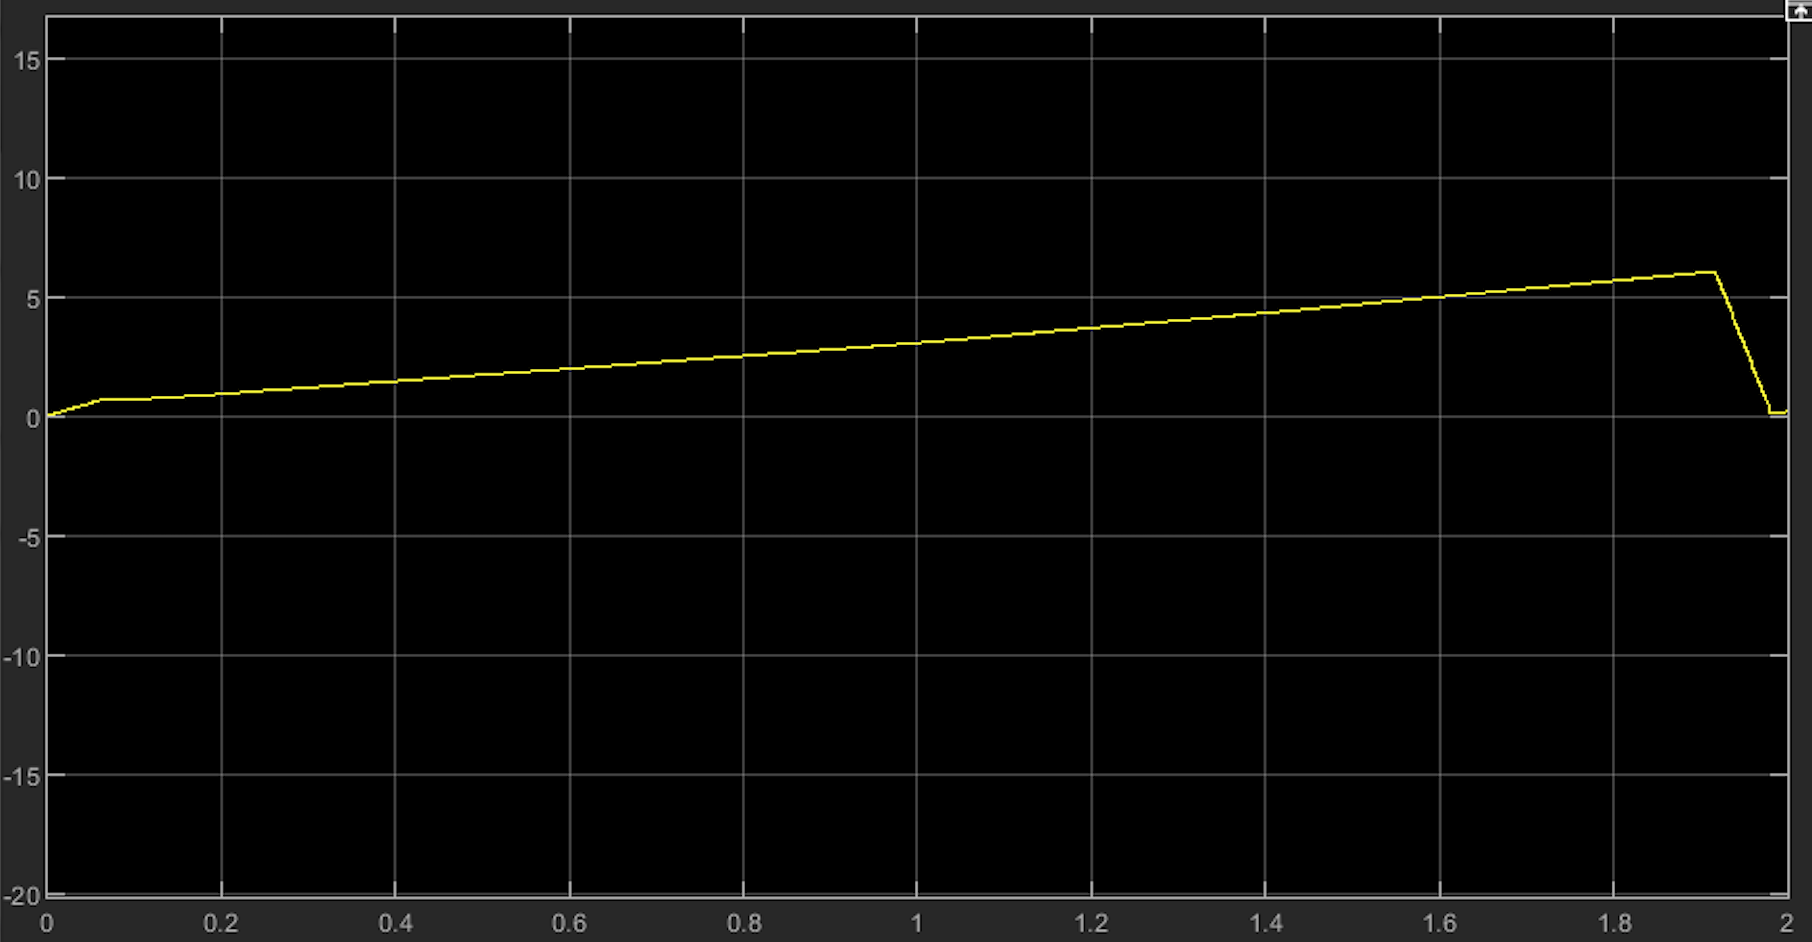
\includegraphics[width=\textwidth]{angle.png}
    \caption{Verlauf der Winkelposition gegenüber der Zeit t [ in Sekunden]}
  \end{minipage}
\end{figure}

\vspace{5mm}
Weieterhin war gefordert, dass die Umlaufzeit auf 2 Sekunden im Uhrzeigersinn eingestellt wird.\\Dies haben wir gelöst, indem wir die Geschwindgikeit des Motors auf $\pi$ eingestellt haben, da:\\
$\frac{Eine Umdrehung}{Zwei Sekunden} = \frac{2\pi}{2sec} = \frac{\pi}{sec}$ in $[\frac{rad}{sec}]$\\
\\Durch Bildung des arithmetischen Mittelwertets haben wir innerhalb der Brownout Grenzen solange die Steuergröße des Motors verstellt bis wir auf eine Winkelgeschwindigkeit von $\frac{\pi}{sec}$ kamen.
Der Verlauf des Positionssignals ist in Figure 4 zu sehen. Dieser ähnelt dem eines Sägezahn-Signals, wobei auffällt, dass das Signal sehr steil von 0 auf $2\pi$ wechselt, da ein Umlauf vollzogen ist und ein Neuer beginnt.
Nach dem Einschwingen lässt sich außerdem festhalten, dass die Zu- bzw. Abnahme fast linear ist.
Die Frequenz des Signals folgt der Einstellung des Drehmomentes und kann durch diese verändert werden. Die maximale und minimale Frequenz erreicht das Signal jeweils durch die Verwendung der Brownout-Grenzwerte.


\newpage


\section{Regelung der oberen Gleichgewichtslage}
\subsection{Beschreibung der Bewegung}
\subsubsection{Differentialgleichungen}
Wir wissen aus der Physik, dass
\begin{equation}\label{eq:physics}
  m \,l^2 \, \ddot{\theta} - m\,g\,l\,\sin{\theta} = \minus M
\end{equation}
wobei $m$ die Masse des Anh\gera ngers, $l$ die L\gera nge des Hebelarms, $g$ die Schwerebeschleunigung und $M$ der Drehmoment bezeichnet. Wir haben das Vorzeichen von $M$ so gew\gera hlt, dass es mit dem Vorzeichen von dem Wert zu dem \textbf{Arduino Continuous Servo Write} passt(siehe unten).\\
\subsubsection{Linearisierung}
Wir benutzen die Standardlinearisierung also $\sin{\theta} \approx \theta$ ist. \\
Linearisierung liefert: 
\begin{equation}\label{eq:linear}
  m \,l^2 \, \ddot{\theta} - m\,g\,l\, \theta = \minus M
\end{equation}
\subsubsection{Laplace Transformation}
Die Laplace-Transformation lautet dann:
\begin{align}\label{eq:laplace}
  m \,l^2 \, s^2 \theta(s) - m\,g\,l\, \theta(s) &= \minus M(s)\\
  \Rightarrow \theta(s) &= \frac{\minus \frac{1}{ml^2}}{s^2 - \frac{g}{l}} M(s)
\end{align}
Die Polstellen sind gegeben durch $\pm \sqrt{\frac{g}{l}}$. 
\subsubsection{Schwingverhalten}
Da eine Polstelle einen positiven Realteil haben, wissen wir, dass das urspr\geru ngliche System nicht stabil ist.\\
\subsection{Herleitung der Regelparameter}\label{section:mathsDerive}
Da wir für die Steuerung von dem Motor nicht den genauen Wert von dem Drehmoment, sondern
eine Zahl mit absoluten Betrag zwischen $0$ bis $90$ für den Block \textbf{Arduino Continuous Servo Write} benutzen 
können, müssen wir noch den Drehmoment in obiger Formel umsetzen. Wir definieren diese Konstante als \textbf{torqueToMotor}.\\
Wir haben in der Dokumentation von dem Motor gefunden dass, der maximale Wert vom Torque $2.5 \text{kg} \cdot \text{cm}$ ist. Also sind wir auf
den Wert (alles in SI-Einheiten) von $\frac{2.5 \cdot g \cdot 0.01}{90} \cdot 5 $ gekommen, wobei $g = 9.8$ die Schwerebeschleunigung bezeichnet.
Zu dem letzten Faktor $5$ haben empirisch gesetzt, damit die Steuerung gewünschte Verhalten liefert. (siehe auch nächste Section)
\subsection{Implementation des Reglers}\label{section:reglerImplement}
Wir benutzen jetzt den matlab Befehl \textbf{place}, um die gewünschte Eigenwerte zu erreichen.\\
Für den weiteren Wert des Parameters in \ref{section:mathsDerive} setzen wir folgendes:
\[
  m = 0.4, \quad piConst = 3.1483, l = 0.15
\]
Wir haben den Wert von $\pi$ so gewählt, da wir gefunden haben, dass bei 
der oberen Gleichgewichtslage der Winkel, der den Motor Block misst, solchen
Wert hat. \\ 
\subsubsection{Reglerparamter des Zustandsreglers}
Wir f\geru hren den Vektor des Zustandsraums ein:
\[
 x := \begin{pmatrix}
  \theta\\
  \dot{\theta}
\end{pmatrix}
\]
und die Gleichung \ref{eq:linear} umformt sich als Folgendes:
\[
\begin{pmatrix}
  \theta\\
  \dot{\theta}
\end{pmatrix} ^{\prime}= 
\begin{pmatrix}
 0 & 1 \\
 \frac{g}{l} & 0
\end{pmatrix}
\begin{pmatrix}
  \theta\\
  \dot{\theta}
\end{pmatrix} - 
\begin{pmatrix}
  0\\
  \frac{T}{m\,l^2}
\end{pmatrix} u
\]
Damit haben wir die Übertragungsfunktion von offenen Regelkreis bestimmt.
\[
	H(s) = (K1 + K2 \cdot s) \, \cdot \frac{\frac{T}{m\,l^2}}{s^2 - \frac{g}{l}}
\]
wobei, $T$ für die Konstante \textbf{torqueToMotor} steht. $u$ ist der Wert f\geru r die Eingabe zu dem Block \textbf{Arduino Continuous Servo Write} ist.\\ 
Sei jetzt $u = (K1, K2)x^{tr}$. Dann gilt nach Laplace Transformation:
\[
  \begin{pmatrix}
    s & -1\\
    -\frac{g}{l} - \frac{T}{m l^2} & s - \frac{T K2}{m l^2}
   \end{pmatrix}
\]
dass die obige Matrix die Eigenwerte davon $5$ und $7$ besitzen. Also
\begin{equation}\label{eq:k12}
  s^2 - \frac{T K2}{ml^2}s - (\frac{g}{l} + \frac{TK1}{ml^2}) = 0
\end{equation}
Wir bekommen den Wert von $K$ mit $K1 = -66.3428$, und $K2 = -7.9347$. 
\subsubsection{Eigenschaft des Zustandreglers}
Da die Zustandregler die Form $(K1 + K2 s)\theta(s)$ hat, sehen wir dass es sich um eine PD-Regler handelt.
\subsubsection{phase margin}
Die Phasenreserve des geschlossenen Regelkreises ist in (Figure \ref{fig:phaseMargin}) geplottet.
\begin{figure}[h]
	\caption{Phasen Reserve von geschlossen Regelkreis}
	\centering
	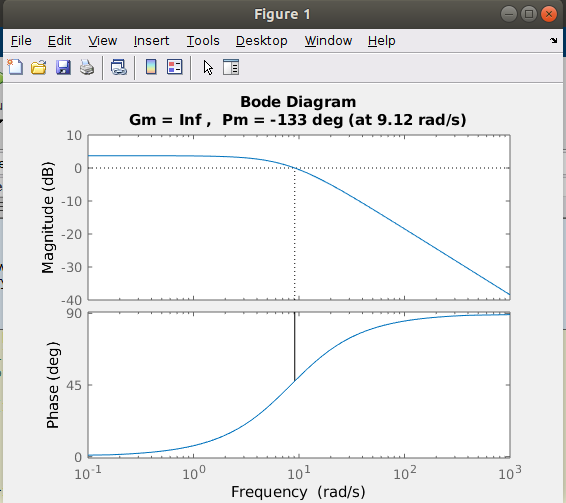
\includegraphics[width=8cm]{phaseMargin}
	\label{fig:phaseMargin}
\end{figure}
Wir haben einen positiven Phasenreserve gesehen also haben wir
ein stabiles System.
\subsubsection{Diskretisierung}
Nun gilt laut Aufgabenstellung, dass $K2$ mit einer $PT1$ Element multipliziert wird. Also
\[
	H(s) = (K1 + \frac{K2 \cdot s}{1 + \tau \cdot s}) \, \cdot \frac{\frac{T}{m\,l^2}}{s^2 - \frac{g}{l}}\quad, \tau = 10^{-2}s
\]
Durch die Transformation $s \mapsto \frac{z - 1}{T}$, mit $T = 10^{-2} s$, wir bekommen die diskrete Darstellung von dem Regler:
\begin{align*}
	H(z) &= K1 + \frac{K2\cdot\frac{z - 1}{T}}{1 + \tau \cdot \frac{z-1}{T}} \\
		&= K1 + K2 \cdot \frac{z - 1}{z}
\end{align*}
Da laut Aufgabenstellung $T = \tau$ ist.
\subsection{Implementierung der Regelung auf dem Arduino}
Der Schaltplan ist im Figure \ref{fig:a239},\ref{fig:a24Sub} gezeigt.\\
\begin{figure}[h]
  \caption{gesamt Schaltplan}
  \centering
  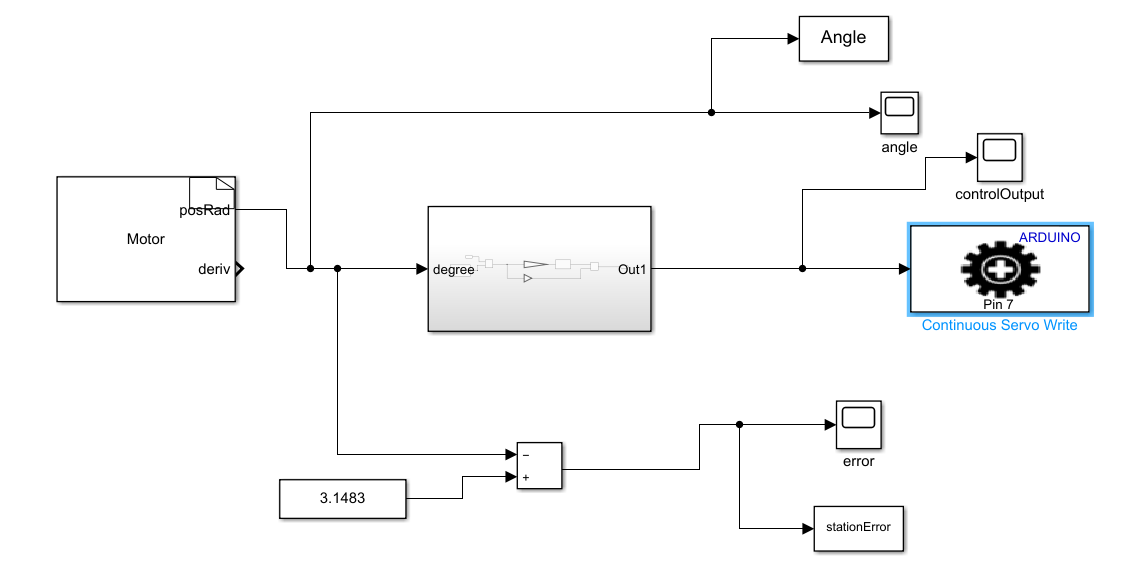
\includegraphics[width=8cm]{images/a239.PNG}
  \label{fig:a239}
\end{figure}
\begin{figure}[h]
  \caption{PD-Regelung}
  \centering
  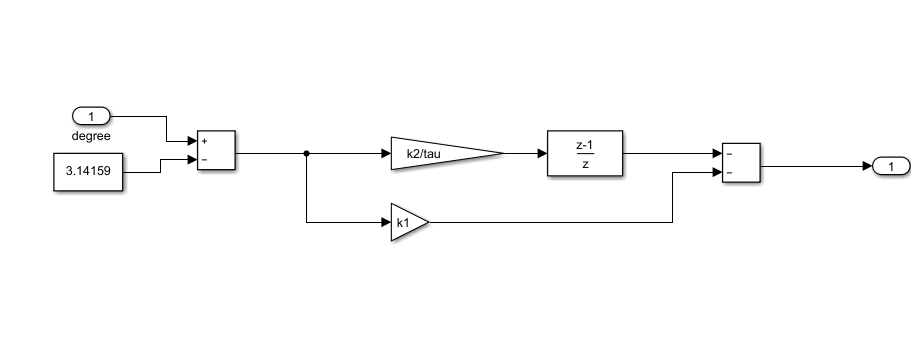
\includegraphics[width=8cm]{a24Sub1}
  \label{fig:a24Sub}
\end{figure}
Wir untersuchen die Regelung auf dem Arduino infolge der in der Aufgabe gestellte Tabelle.\\
Da wir nur $9$ Große Unterlagscheiben haben, haben wir bis Konfiguration $5$ gearbeitet. \\
Die geneauere Beschreibung befindet sich in der folgenden Tabelle. \\
\begin{center}
  \begin{tabular}{ |c|c|c|}
    \hline
    Konfiguration & Verhalten & stationärer Fehler \\
    \hline
    1 & sehr schnell zur Ruhrlage & 0.006 \\
    \hline
    2 & schnell zur Ruhrlage & 0.0071 \\
    \hline
    3 &  \shortstack{wackelt um das Gleichgewichtslage \\ aber die Amplitude klingt schnell ab} & 0.025 \\
    \hline
    4 & wackelt langsamer als 3 zur Ruhrlage & 0.045 \\
    \hline
    5 & wackelt langsamer als 4 zur Ruhrlage & 0.016 \\
    \hline
  \end{tabular}
\end{center}
\subsection{station\gera re Fehler}
Wir haben in der oberen Tabelle gesehen, dass es immer station\gera re Fehler auftreten. Grund daf\geru r kann m\gero glich sein, dass die Reibung drinnen in dem Motor verhindert, diese kleine Bewegung zu steuern. Ein anderer Grund ist wegen des Fehlers die auftreten waehrend der Linearisierung und Diskretisierung. Wir haben gesehen, dass am Ende das Pendel immer nur wenig hin und her wackelt aber nicht zu einer kompletten Ruhelage, also kann sein, dass der Schrittweite, die das Signal abgetastet wird nicht fein genug ist. \\
Wir haben auch versucht, vor dem Regler ein Integrator zu integerieren aber hilft dies auch nicht. Leider muessen wir uns mit dem stationaeren Fehler leben.

\section{Aufschwingen des Pendels}
\subsection{Aufbauen der Regelung}
Um das Pendel aus der unteren Gleichgewichtslage zu der oberen Gleichgewichtslage zu führen,
benutzen wir zuerst den bereitgestellten bang-bang Control Block, damit wir den Hebelarm bis zu
einem Winkel hochheben, so dass wir mit der vorher gebildeten Regelung das Pendel zur oberen Gleichgewichtslage
steuern können. \\
Wir führen hier ein Switch ein. Der entscheidet den Winkel zwischen der der Motor Block misst (der aktuelle Winkel) und
der Sollwert (3.1483, siehe section \ref{section:reglerImplement}). Falls der Fehler unter einer Grenze liegt, dann nutzen wir die PD-Regelung
um das System weiter zu steuern.  Wir haben w\gera hrend des Experiments entdeckt, dass bei Nullpunktdurchgang wegen des abrupter \"{A}nderung von $0$ bis $2 \pi$ \gera durch Interpolation ein Wert sehr nahe bei $\pi$ liegen, also in diesem Fall falsch die PD-Regelung starten wird. Deswegen haben wir eine Verz\gero gerungsglied hinzugef\geru gt um dieses Problem zu beheben. Durch die Verz\gero gerung vergleichen wir den aktuellen Winkel mit dem Wert vor $10$ abgetasteten Wert. Wenn der abrupt \gera ndert, wissen wir dass ein Nullpunktdurchgang auftritt also verwerfen diese Situation, ansonsten ist starten wir die PD-Regelung.(siehe den Schaltplan in Section \ref{section:last})
%\bibliographystyle{plain}
%\bibliography{references}
\subsection{Bereich der PD-Regelung}
Wir haben empirisch bestimmt, dass der Winkel zwischen 0.3 bis 2 ist.
\subsection{maxTorque und minTorque}
Das haben wir in der Aufgabe 2.2 schon bestimmt.
\subsection{Verhalten des Systems}\label{section:last}
Hier unten ist ein Screenshots von dem Schaltplan.
\begin{figure}[h]
  \caption{Schaltplan vom Aufschwingen}
  \centering
  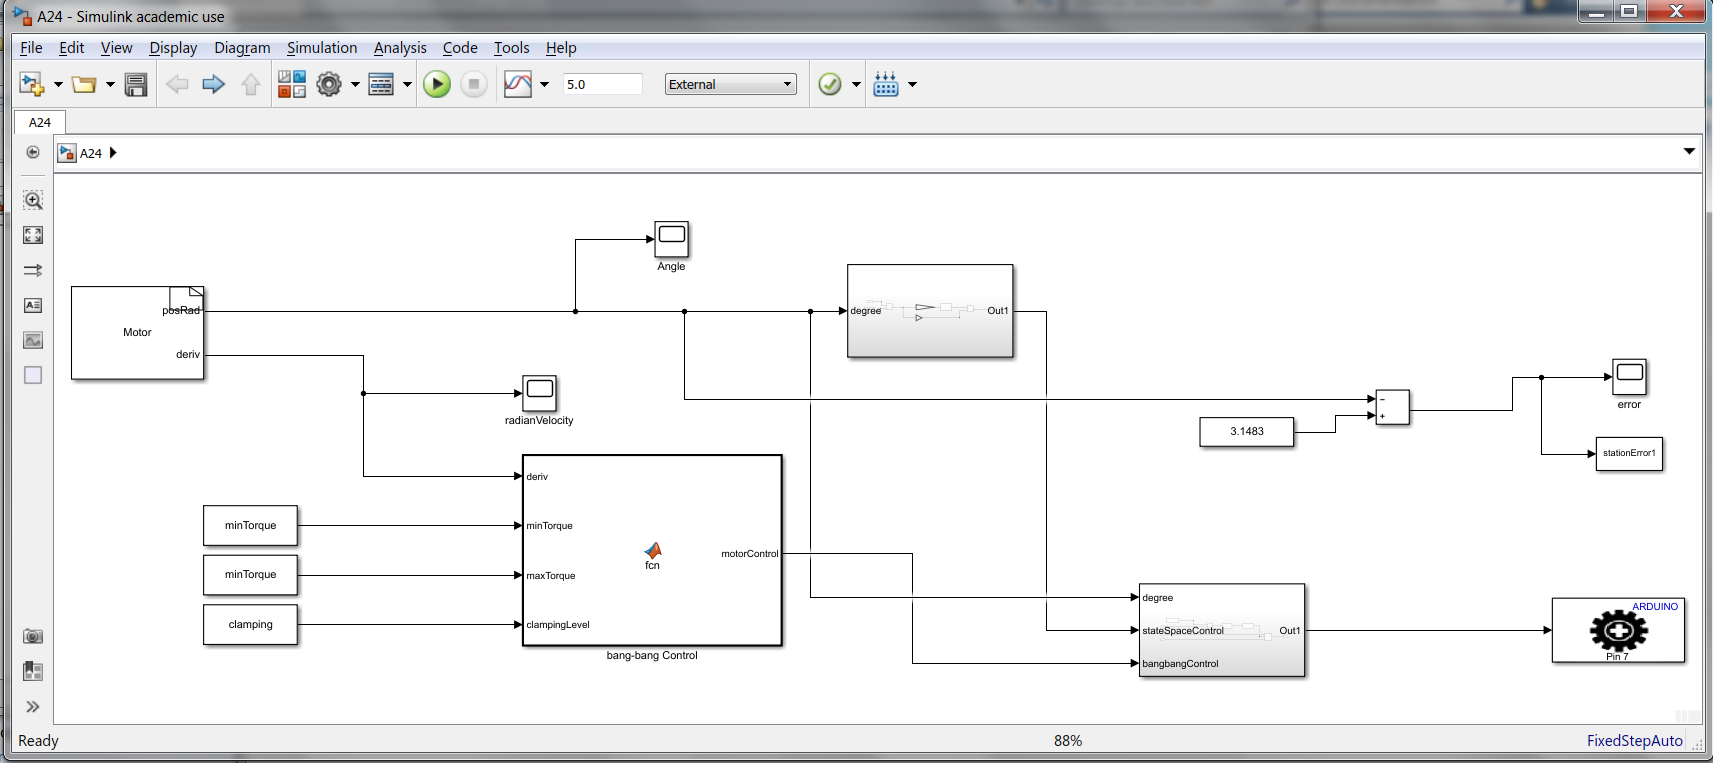
\includegraphics[width=10cm]{a24}
  \label{fig:schaltplan24}
\end{figure}\\
Für das Subsystem sieht der Schaltplan so aus.
\begin{figure}[h]
  \caption{switch Block}
  \centering
  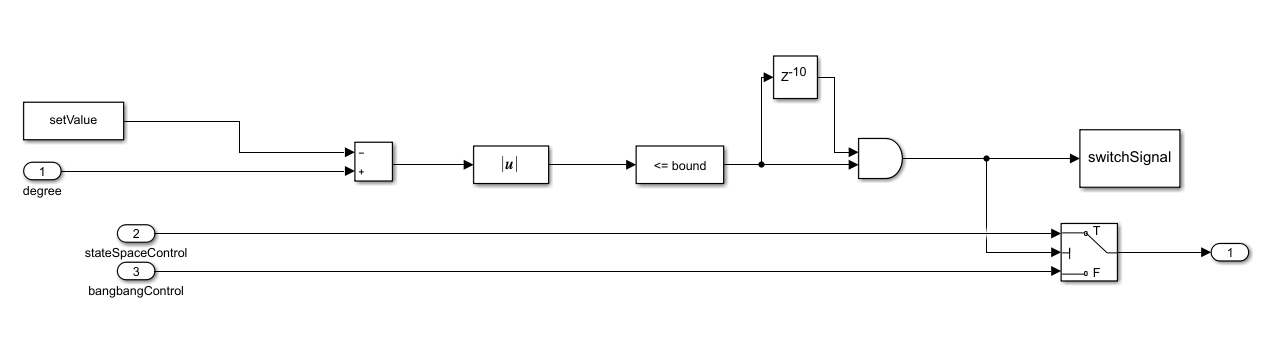
\includegraphics[width=8cm]{switch}
  \label{fig:switch}
\end{figure}
\begin{figure}[h]
  \caption{PD-Regelung}
  \centering
  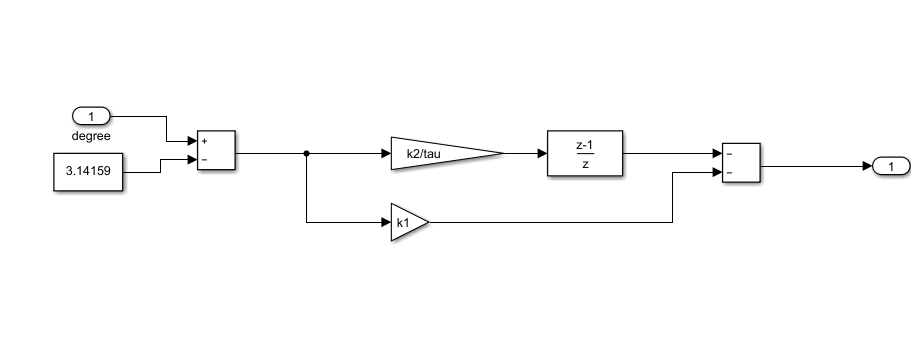
\includegraphics[width=8cm]{a24Sub1}
  \label{fig:pdRegelung}
\end{figure}\\
Bei der Durchf\geru hrung vom Experiment haben wir das folgende Ergebnis:
% \begin{figure}[h]
%   \caption{deriv}
%   \centering
%   \includegraphics[width=8cm]{images/radianSpeed.PNG}
%   \label{fig:rSpeed}
% \end{figure}
% \begin{figure}[h]
%   \caption{posRad}
%   \centering
%   \includegraphics[width=8cm]{images/Angle1.PNG}
%   \label{fig:pdRegelung}
% \end{figure}
% \begin{figure}[h]
%   \caption{switchSignal}
%   \centering
%   \includegraphics[width=8cm]{images/switchSignal.PNG}
%   \label{fig:switchSignal}
% \end{figure}
\begin{figure}[h]
  \centering
  \begin{minipage}[b]{0.4\textwidth}
    \includegraphics[width=\textwidth]{radianSpeed.PNG}
    \caption{deriv}
  \end{minipage}
  \hfill
  \begin{minipage}[b]{0.4\textwidth}
    \includegraphics[width=\textwidth]{Angle1.PNG}
    \caption{posRad}
  \end{minipage}
  \hfill
  \begin{minipage}[b]{0.4\textwidth}
    \includegraphics[width=\textwidth]{switchSignal.PNG}
    \caption{switch signal}
  \end{minipage}
\end{figure}
Wir sehen dass der Abschwingvorgang ziemlich kurz ist, danach 
wird die PD-Regelung aufwirken und steuert das Pendel zur oberen
Gleichgewichtslage.
\end{document}
